% Build with pdfLaTeX: pdflatex main && bibtex main && pdflatex main && pdflatex main (or Overleaf, pdfLaTeX).
% Tables in tables/ are generated by `uv run python -m src.tables`; figures are written by the notebooks, except fig-rolling-pr-reliability-budget (`uv run python -m src.plotting`).

\documentclass[conference]{IEEEtran}
\usepackage{cite}
\usepackage{amsmath,amssymb,amsfonts}
\usepackage{graphicx}
\usepackage{booktabs}
\usepackage{xcolor}
\usepackage{url}
\def\UrlBreaks{\do\/\do-\do.\do_\do=}
\usepackage{textcomp}
\usepackage{float}
\usepackage{array}
\newcolumntype{R}[1]{>{\raggedright\arraybackslash}p{#1}}
\usepackage{tikz}
\usetikzlibrary{arrows.meta,positioning,shapes.geometric}
\graphicspath{{figures/}}
% Float-only pages start at the top instead of centring their floats.
\makeatletter
\setlength{\@fptop}{0pt}
\setlength{\@fpsep}{12pt plus 2fil}
\setlength{\@fpbot}{0pt plus 1fil}
\makeatother
\hyphenation{Hima-laya anti-ci-pa-tory re-ana-ly-sis}
\newif\ifieeebold \ieeeboldfalse % set \ieeeboldtrue for IEEE's default bold abstract
% Abstract and index-terms body in normal weight; the run-in labels keep IEEEtran's style.
\newcommand{\abstractbody}{\ifieeebold\else\normalfont\fi}
\usepackage[hidelinks]{hyperref}
\hypersetup{pdftitle={Analysis and Prediction of Monsoon Hazards in Nepal Using Machine Learning Approaches},pdfauthor={Bhimraj Yadav}}
% Code link (Appendix A).
\newcommand{\codeurl}{\url{https://github.com/bhimrazy/st7072cem-ml-assignment}}

\begin{document}

\title{Analysis and Prediction of Monsoon Hazards in Nepal Using Machine Learning Approaches}

\author{\IEEEauthorblockN{Bhimraj Yadav}
\IEEEauthorblockA{\textit{ST7072CEM Machine Learning}\\
Softwarica College of IT and E-Commerce, in collaboration with Coventry University\\
Kathmandu, Nepal\\
Coventry University Student ID: 17624402\\
260177@softwarica.edu.np}}

\maketitle

\begin{abstract}
\abstractbody
Floods, landslides, heavy rainfall and lightning kill more than a hundred people in Nepal every year; in late September 2024, three days of record rain alone killed 249 and blocked the main highways into Kathmandu. Nepal's new anticipatory action framework will release relief before disasters strike once triggers (pre-agreed forecast conditions) are met. That needs forecasts of when harm is likely, not only of where hazards can occur, yet machine-learning work in Nepal has mostly mapped susceptibility. This study forecasts, for each of the 77 districts and each day from April to October, whether a damaging incident (a death, missing person, injury or destroyed house) will be recorded in the next three days. The dataset joins the official disaster record (BIPAD) with ERA5 reanalysis rainfall: 146,223 district-days for 2017 to 2025, 6.8\% positive. K-means, Ward and Gaussian mixture clustering group districts into risk regions. Logistic regression, random forest, gradient boosting and support vector machines are tuned with season-blocked cross-validation, and each test season is scored by models fitted on all earlier seasons. District-by-month climatology scores 0.151 in mean per-season precision-recall AUC (PR-AUC); three of five models gain about 0.026 (lower bounds near 0.005), all in 2024. In 2025 and a 2026 check none clearly beats climatology. The regions are interpretable but add nothing to a pooled model. A perfect three-day rain forecast raises PR-AUC to about 0.21, more than the model spread, mostly in 2024. Reporting bias and lightning are the main caveats.
\end{abstract}

\begin{IEEEkeywords}
\abstractbody
impact-based forecasting, machine learning, clustering, landslides, floods, lightning, Nepal
\end{IEEEkeywords}

\section{Introduction}
Nepal's monsoon brings most of the country's annual rain between June and September. From 2017 to 2025, BIPAD records 2,561 deaths from floods, landslides, heavy rainfall and lightning, at least 112 each year \cite{BIPAD2026}. In June 2021, heavy rain and snowmelt above Melamchi set off landslides, a temporary river dam and a debris flood that left about 25 people dead or missing and wrecked the headworks of Kathmandu's new water supply \cite{Maharjan2021Melamchi,Duwadi2024}. In June 2023, flash floods in Sankhuwasabha, Taplejung and Panchthar swept away workers at hydropower sites \cite{KathmanduPost2023East}. On 12 July 2024, a landslide at Simaltal pushed two buses carrying about 60 people into the Trishuli \cite{KathmanduPost2024Simaltal}. From 26 to 28 September 2024, a stalled low-pressure system brought record rain to central and eastern Nepal. It killed 249 people and blocked the main highways into Kathmandu, and a debris flow at Jhyaple Khola killed 35 people in queued vehicles \cite{NDRRMA2024LossDamage,Lamichhane2025,Petley2025}. On 11 October 2026, a flood from a suspected landslide dam on the Budhi Gandaki in Gorkha struck on a dry day \cite{KathmanduPost2026,AlJazeera2026}.

In each, harm came from several hazards at once, sometimes far from the heaviest rain, within days of the rain that set it off. Extreme rainfall has increased at many stations, with spatially mixed trends \cite{Karki2017,Talchabhadel2018,IPCC2021Ch11}. The Himalayan arc holds a large share of the world's fatal landslides \cite{Petley2012,FroudePetley2018}, and road building adds exposure, as at Simaltal \cite{MunozTorrero2021,KathmanduPost2024Simaltal}. Nepal's National Anticipatory Action Framework (2026) aims to release relief before a hazard strikes, with forecasts and triggers (pre-agreed forecast conditions) as one of its three building blocks \cite{NDRRMA2026}. For a district administration deciding whether to pre-position relief, the useful trigger is a forecast of impact: whether people are likely to be hurt in the next few days, whatever the mechanism.

Machine learning in Nepal has mostly produced static susceptibility maps, of landslides from inventories and terrain \cite{Kincey2024} and of multiple hazards, some under climate scenarios \cite{Thapa2026,Shrestha2026}. They show where hazards can occur but not when. Rainfall thresholds supply timing, but for slope failure alone \cite{Dahal2008,Guzzetti2020}. Machine-learning impact forecasts exist for single hazards in data-rich settings, such as global landslide nowcasting \cite{Stanley2021}, severe-weather and flood impacts in Catalonia \cite{Iglesias2024,Morales2026}, and tropical-cyclone housing damage \cite{KooshkiForooshani2024}. The impact module of BIPAD, Nepal's national disaster portal, was prototyped for riverine floods at two stations \cite{UNDRR2025}. To the author's knowledge, no published model forecasts, district by district and day by day, whether any of the main monsoon hazards will cause casualties or destroy homes in Nepal. A second gap is methodological. Nepal's districts range from the Terai plain to the high Himalaya, so a single national model may hide where it fails, yet in hydrology pooled models trained on all sites often beat regional ones \cite{Kratzert2019,Fang2022}. Whether learned regions help a harm forecast has not been tested.

This study builds and evaluates a daily, district-level harm forecast for Nepal's monsoon hazards from open data. The objectives are: (1) to cluster districts into monsoon risk regions with similar impact history and rain climate; (2) to classify whether a district will suffer a damaging hydro-meteorological incident in the next three days; and (3) to test whether the regions improve prediction, and to explain which factors drive risk. A damaging incident is one that records at least one death, missing person, injury or destroyed house.

The first contribution is a harm dataset from BIPAD whose unit is the district-day (one district on one day), with recording changes made explicit and leakage checked. The second is a fair test of whether learned regions help, against the climatology (historical district-month rate), persistence and threshold baselines a forecaster would use. The third is an analysis of where and why the forecast fails, by region, hazard and month. Two bounds, no weather and a perfect rain forecast, separate the value of rainfall information from that of the model.

\section{Related Work}
A hazard forecast says whether a physical event is likely; an impact forecast says what it will do to people and assets \cite{Merz2020}. Impact-based warnings aim at the second \cite{Potter2025}, and anticipatory action uses them to release funds before an event \cite{CoughlanDePerez2015}. Monsoon harm in Nepal is multi-hazard in the sense of Gill and Malamud \cite{GillMalamud2014}. Floods, landslides and heavy rain share a driver and often coincide, while lightning shares the season but not the mechanism, a framing increasingly adopted in risk research \cite{Zscheischler2018,Ward2022,Ferrario2026,Jager2025}. A target built from damaging incidents is a harm label: it folds hazard, exposure and vulnerability together as recorded, which suits an anticipatory trigger but makes the label sensitive to reporting.

\subsection{Rainfall Thresholds and Early Warning}
Intensity-duration thresholds for landslide initiation are the oldest operational tool \cite{Guzzetti2008,Segoni2018,Guzzetti2020}. For Nepal, Dahal and Hasegawa fitted $I = 73.90\,D^{-0.79}$ (mm/h over $D$ hours) to 193 landslides, which gives about 144 mm/day \cite{Dahal2008,Dahal2008Erratum}. Thresholds are transparent, but they say nothing about whether anyone is hurt. They also transfer poorly from rain gauges to the coarse grid of a reanalysis, a model reconstruction of past weather. This study uses the Nepal threshold as a baseline and, for fairness, refits a percentile threshold on ERA5 rain.

\subsection{Machine Learning Hazard Mapping in Nepal}
Reichenbach et al. reviewed statistical susceptibility mapping and its reliance on inventories \cite{Reichenbach2018}. Kincey et al. mapped rainfall-triggered landslide susceptibility and exposure for Nepal, showing that susceptibility peaks in the High Himalaya but exposure in the Middle Hills \cite{Kincey2024,Kincey2023Data}. Thapa et al. cluster Nepal into zones with K-means on static susceptibility layers \cite{Thapa2026}, and Shrestha et al. assess compound flood-landslide and drought-fire interactions under CMIP6 scenarios \cite{Shrestha2026}. These studies locate hazard; none forecasts daily harm. Since Thapa et al. already cluster Nepal, clustering in this study is a means to test whether regions help a forecast.

\subsection{Forecasting Occurrence and Impact with Machine Learning}
Stanley et al. turned NASA's landslide hazard assessment into a data-driven global nowcast \cite{Stanley2021}. Their XGBoost model uses antecedent rain and static factors and is trained on inventories with a temporal hold-out. Doerksen et al. predict landslides by district in Nepal over 7, 10 and 14-day windows, using random forests and U-Nets on satellite precipitation and geomorphic data \cite{Doerksen2023}. Dahal et al. model landslide occurrence and density in space and time for the Gorkha-affected region \cite{DahalA2024}, the closest Nepal comparator.

Impact forecasting from impact records is most developed in Korea, where heavy-rain damage is classified from daily weather \cite{Choi2018,Kim2019a,KOSHAM2025}, and in Catalonia, where Iglesias et al. predict severe-weather impact on people at municipality-day level and beat the official warning \cite{Iglesias2024}. Morales et al. predict flood-related emergency calls per municipality and hour, with walk-forward evaluation and separate models per population-density group \cite{Morales2026}. Operational anticipatory-action triggers are event-based. Kooshki Forooshani et al. took the housing-damage model that triggers anticipatory action for tropical cyclones in the Philippines to global scale \cite{KooshkiForooshani2024}, and Sedhain et al. show that such triggers can have very low detection on a real typhoon \cite{Sedhain2025}. This study therefore reports detection and false alarms at a fixed alert budget (a cap on the share of district-days alerted). Table~\ref{tab:closest} compares the closest works. None combines several hazards, a daily horizon and a national loss record for Nepal.

\begin{table}[t]
\caption{Closest works. Forecasting rows with a known design use time-ordered evaluation; the Doerksen et al. and Dahal et al. rows come from their abstracts.}
\label{tab:closest}
\centering
\scriptsize
\setlength{\tabcolsep}{3pt}
\begin{tabular}{R{1.65cm}R{1.65cm}R{1.4cm}R{1.55cm}R{1.45cm}}
\toprule
Study & Unit, horizon & Hazards & Label & Baseline \\
\midrule
Stanley et al. 2021 \cite{Stanley2021}, global & 30 arc-second (about 1 km) grid, daily nowcast & Landslide & Landslide inventories & LHASA 1.0 \\
Doerksen et al. 2023 \cite{Doerksen2023}, Nepal & District, 7, 10 and 14-day windows & Landslide & Landslide occurrence & RF and U-Net compared; thresholds critiqued \\
Dahal et al. 2024 \cite{DahalA2024}, Gorkha region & 1 km cell, about 6-month periods & Landslide & Occurrence and areal density & Not in abstract \\
Iglesias et al. 2024 \cite{Iglesias2024}, Catalonia & Municipality, daily & Severe weather & Emergency-incident counts & Official warning \\
Morales et al. 2026 \cite{Morales2026}, Catalonia & Municipality, next hour & Flood & 112 emergency calls & Climatology-based warnings \\
Kooshki Forooshani et al. 2024 \cite{KooshkiForooshani2024}, Philippines & Municipality and 0.1\textdegree{} grid, per event & Tropical cyclone & Humanitarian damage data, 39 typhoons & Earlier operational model \\
Thapa et al. 2026 \cite{Thapa2026}, Nepal & District and grid, static & Flood, landslide & Susceptibility layers & None \\
This study, Nepal & District, 3 days & Flood, landslide, heavy rain, lightning & BIPAD loss record & Climatology, persistence, thresholds \\
\bottomrule
\end{tabular}
\end{table}

\subsection{Disaster Loss Records and Their Biases}
Loss databases under-record small and remote events, and their coverage changes over time, so trends in recorded losses mix changes in hazard, exposure and reporting \cite{Gall2009,Jones2022}. In Nepal, recorded lightning deaths rose with internet access \cite{Adhikari2021}, and Harvey et al. find large gaps in Nepal's landslide inventories \cite{Harvey2024}. BIPAD is the Government of Nepal's incident portal, maintained by the National Disaster Risk Reduction and Management Authority (NDRRMA) \cite{BIPAD2026,Gyawali2022}. It is the only national, incident-level source with locations and losses, so these biases shape what any model can learn.

\section{Problem and Dataset}
\subsection{Study Area and Season}
\label{sec:area}
\begin{figure}[t]
\centering
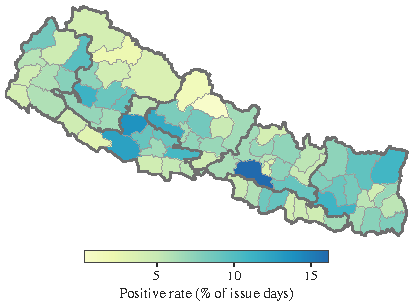
\includegraphics[width=\columnwidth]{fig-district-rate-map-a.pdf}
\caption{Positive rate (damaging incident within three days) by district, 2017 to 2025. Boundaries: OCHA COD-AB \cite{OCHA2026COD}; belts in Fig.~\ref{fig:belts}.}
\label{fig:studymap}
\end{figure}
Nepal's 77 districts span three ecological belts within 200 km: the Terai plain below 300 m, the Hill belt of the Mahabharat and Middle Hills, and the Mountain belt above 3,000 m. The belts are approximated from elevation: a district is Mountain if its mean ward elevation is at least 1,700 m and at least 5\% of its wards lie above 3,000 m, Terai if the mean is below 700 m and fewer than 15\% of wards lie above 1,000 m, and Hill otherwise. Rainfall is strongly orographic and varies across the country \cite{Kansakar2004}. Issue days, at the end of which a forecast is made, run from 1 April to 28 October so that the three-day target window stays inside April to October. The pre-monsoon months are included because the lightning season runs from March to August \cite{Sharma2022} and lightning harm in BIPAD peaks in April and May, while floods, landslides and heavy-rain damage peak in July and August (Fig.~\ref{fig:seasonality}, appendix).

\subsection{Target Data: the BIPAD Incident Record}
No Kaggle, UCI or other public dataset has district-day multi-hazard harm labels for Nepal, so the label is built from the official national record, a snapshot of the BIPAD incident API taken on 19 September 2026, holding 63,549 incidents of all types \cite{BIPAD2026}. Of these, 16,790 records dated 2011 to 2026 have the hazard title Flood, Landslide, Heavy Rainfall or Thunderbolt and are kept. BIPAD itself links each incident to a ward. The ward, municipality and district tables were downloaded once, with their dates, so each incident's district cannot change when the portal updates. Every incident maps to a district. Timestamps are converted to Nepal time and truncated to the calendar day. The loss fields are used only to set the damaging flag and are dropped before any feature is built.

The record has two entry periods. Incidents from 2016 to 2019 were entered in bulk years later, with a median entry lag of 930 days for 2017 incidents. From 2020 the median lag is one day and 94\% of incidents are entered within three days. Recent-incident features may therefore use only what was entered by the issue day. Reporting also grew: between 2017 and 2024 the share of district-days with any recorded incident rose 2.8 times, but the share with a damaging incident rose only 1.4 times (Fig.~\ref{fig:peryear}, appendix). Because the growth concentrates in minor incidents, the target is restricted to damaging ones.

\subsection{Predictors}
Daily weather is ERA5 reanalysis \cite{Hersbach2020} from the Open-Meteo historical API \cite{Zippenfenig2023} at each district centroid, for 2 March to 31 October of 2016 to 2026 (2026 to 31 August; 201,971 district-days, no gaps). The variables are precipitation sum, precipitation hours and maximum temperature in Nepal time. ERA5 has a 0.25\textdegree{} grid, so each district is one point and orographic peaks are smoothed. Terrain is summarised from the elevations of all 6,803 ward centroids (Copernicus DEM through Open-Meteo) as district mean elevation, elevation range and the share of wards above 1,000 m and 3,000 m.

\subsection{Problem Definition and Sampling}
The unit is a district $d$ on an issue day $t$. With $D_{d,\tau}=1$ if district $d$ has at least one damaging incident of the four hazards dated day $\tau$, the primary, all-hazard target is
\begin{equation}
y_{d,t} = \max\left(D_{d,t+1},\, D_{d,t+2},\, D_{d,t+3}\right).
\label{eq:target}
\end{equation}
A three-day window matches a short anticipatory-action lead time and absorbs the day-level uncertainty of incident records. Secondary labels take the same form for each hazard, for fatal incidents, and for the rain-driven hazards alone (flood, landslide and heavy rainfall, $y_{\mathrm{rain}}$). The panel of all district-days holds 77 districts and 211 issue days per season for 2017 to 2025: 146,223 rows, 9,953 of them positive ($y=1$, 6.81\%). Lightning is part of 38\% of positive rows and the only hazard in 36\% of them. The 2026 season is an out-of-time check; its issue days stop at 16 August, so the last window ends 31 days before the snapshot. Evaluation uses an expanding window over whole seasons (Table~\ref{tab:splits}): 2024 is scored by models fitted on 2017 to 2023, 2025 on 2017 to 2024 and the 2026 check on 2017 to 2025.

\begin{table}[t]
\caption{Expanding-window schedule: the training seasons of each scored season, with rows and positive rates.}
\label{tab:splits}
\centering
\scriptsize
\setlength{\tabcolsep}{3pt}
\begin{tabular}{llrrrrr}
\toprule
 & & \multicolumn{2}{c}{Training} & \multicolumn{3}{c}{Scored} \\
\cmidrule(lr){3-4}\cmidrule(lr){5-7}
Scored & Fitted on & Rows & $y$ (\%) & Rows & Pos. & $y$ (\%) \\
\midrule
2024 & 2017--2023 & 113,729 & 6.33 & 16,247 & 1,466 & 9.02 \\
2025 & 2017--2024 & 129,976 & 6.67 & 16,247 & 1,283 & 7.90 \\
2024--25 & per season & & & 32,494 & 2,749 & 8.46 \\\addlinespace[2pt]
2026 check & 2017--2025 & 146,223 & 6.81 & 10,626 & 614 & 5.78 \\
\bottomrule
\end{tabular}

\end{table}

\subsection{Data Quality}
Within a district, consecutive issue days share two of their three target days, so $y$ has a lag-one autocorrelation of about 0.69, and one storm can hit many districts on the same day (36 on 28 September 2024). Tuning folds and bootstrap blocks are therefore whole seasons and weeks.

\section{Methods and Experimental Setup}
\subsection{Design}
Fig.~\ref{fig:pipeline} shows the two-stage design. Stage 1 clusters the districts into risk regions from their 2017 to 2022 profiles, and Stage 2 trains models on the district-day panel with and without the regions as features. The regions enter one pooled model as extra features; no per-region models are fitted. Since set A (below) already holds district-by-month history, the regions can help only if they carry information that history lacks. In hydrology, models trained on many catchments learn regional behaviour on their own \cite{Kratzert2019,Fang2022}. Piernik and Morzy found that a bare cluster label is the weakest way to pass cluster information to a model and that tree ensembles rarely benefit \cite{Piernik2021}. A null result for objective 3 would therefore be informative. The expectation was recorded before the test seasons were scored: if regions helped at all, they would help logistic regression more than the trees.

\begin{figure}[t]
\centering
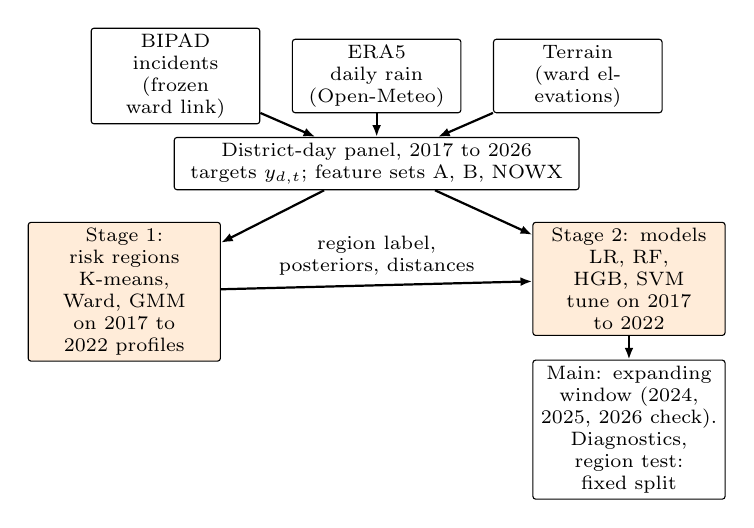
\begin{tikzpicture}[font=\scriptsize, node distance=3mm and 4mm,
  box/.style={draw, rounded corners=1pt, align=center, minimum height=5.5mm, inner sep=2pt, text width=20mm},
  stage/.style={box, fill=orange!15, text width=23mm},
  arr/.style={-{Latex[length=1.5mm]}, thick}]
\node[box] (bipad) {BIPAD incidents\\(frozen ward link)};
\node[box, right=of bipad] (era5) {ERA5 daily rain\\(Open-Meteo)};
\node[box, right=of era5] (dem) {Terrain\\(ward elevations)};
\node[box, below=of era5, text width=50mm] (panel) {District-day panel, 2017 to 2026\\targets $y_{d,t}$; feature sets A, B, NOWX};
\node[stage, below left=4mm and -6mm of panel] (s1) {Stage 1: risk regions\\K-means, Ward, GMM\\on 2017 to 2022 profiles};
\node[stage, below right=4mm and -6mm of panel] (s2) {Stage 2: models\\LR, RF, HGB, SVM\\tune on 2017 to 2022};
\node[box, below=of s2, text width=23mm] (eval) {Main: expanding window (2024, 2025, 2026 check). Diagnostics, region test: fixed split};
\draw[arr] (bipad) -- (panel); \draw[arr] (era5) -- (panel); \draw[arr] (dem) -- (panel);
\draw[arr] (panel) -- (s1); \draw[arr] (panel) -- (s2);
\draw[arr] (s1) -- node[above, align=center] {region label,\\posteriors, distances} (s2);
\draw[arr] (s2) -- (eval);
\end{tikzpicture}
\caption{Two-stage cluster-then-classify pipeline with the time-ordered evaluation.}
\label{fig:pipeline}
\end{figure}

\subsection{Stage 1: Regionalisation}
\label{sec:stage1}
Each district is described by 37 numbers from the seasons 2017 to 2022 only. They are the monthly rate of damaging days for each hazard (4 hazards $\times$ 7 months), the monthly mean daily ERA5 rain (7) and two terrain values; no exposure or vulnerability layer is used. The profile uses same-day rates, so it describes history and does not contain the forecast target. The columns are standardised and reduced by principal component analysis (PCA). The first four components carry 49\% of the variance and each later one adds less than 6\%, so these four form the clustering space. The 19-component space that reaches 90\% is a sensitivity check.

K-means \cite{Lloyd1982} with 50 restarts, Ward's agglomerative clustering and a diagonal Gaussian mixture model \cite{Fraley2002} are fitted for $k = 2$ to 8. Validity is scored with the silhouette \cite{Rousseeuw1987}, Davies--Bouldin \cite{Davies1979} and Calinski--Harabasz \cite{Calinski1974} indices and the mixture's BIC. The rule for $k$ was fixed in advance: among K-means solutions whose smallest region has at least five districts, take the best silhouette, with Davies--Bouldin as tie-break. Stability is the adjusted Rand index (ARI) \cite{Hubert1985} between the reference labels and labels refitted on 200 bootstrap resamples of the six seasons. The same index measures agreement with the ecological belts and the seven provinces.

Following Piernik and Morzy \cite{Piernik2021}, the regions are passed to Stage 2 in three forms: the K-means label (one-hot), the mixture's posterior probabilities and the distances to the K-means centroids.

\subsection{Stage 2: Classification}
Four classifier families are compared, all in scikit-learn \cite{Pedregosa2011}: logistic regression \cite{Hosmer2013} on standardised inputs, random forest \cite{Breiman2001}, histogram gradient boosting \cite{Friedman2001}, and support vector machines (SVMs). The SVMs are a linear SVM on all rows and an RBF SVM on a stratified subsample of 12,000 rows. Linear discriminant analysis and naive Bayes were excluded because the heavy-tailed, correlated rain totals break their assumptions, and k-nearest neighbours because it scales poorly to nearly 100,000 mixed-feature rows. Class imbalance is handled with class weights, since resampling distorts calibrated risk \cite{vandenGoorbergh2022}. Hyperparameters (Table~\ref{tab:hyper}, appendix) are tuned on leave-one-season-out folds within 2017 to 2022, following the season-blocked logic of Roberts et al. \cite{Roberts2017}. The tuning score is mean PR-AUC, the area under the precision-recall curve (Section~\ref{sec:metrics}). For each scored season the models, with these settings fixed, are refitted on all earlier seasons from 2017, as are the rain percentiles, history rates, synthetic entry lags and climatology. Isotonic regression, fitted on leave-one-season-out scores within those seasons (each fold with its own rebuilt features), maps the score to a probability, so no season is held back for calibration; fold models see one season fewer. The diagnostic analyses of Sections~\ref{sec:ablations} to \ref{sec:case} instead use a fixed split: one fit on 2017 to 2022, with 2023 for calibration. Their ``best model'' is the one with the highest tuning PR-AUC, chosen before the test seasons were scored: the random forest, 0.009 behind logistic regression under the expanding window.

Three feature sets are used (Table~\ref{tab:features}, appendix). Set A holds what is known at the end of day $t$: ERA5 rain over 1 to 30 days, an antecedent index and the district percentile of 3-day rain, rain hours, maximum temperature, season, terrain, damaging incidents known at $t$ in the district and its neighbours, and shrunken district-by-month history rates per hazard. ERA5 is released days after the fact, so set A is a hindcast that assumes a perfect same-day weather analysis. Set B adds the observed ERA5 rain for $t+1$ to $t+3$, a perfect-forecast ceiling at ERA5 resolution. NOWX (no weather) drops every weather column and is the floor. NOWX to A measures the value of rainfall information, and A to B the value of a perfect three-day rain forecast.

\subsection{Baselines}
Five baselines are scored:
\begin{itemize}
\item climatology, the district-by-month positive rate of the training seasons, which is also the reference for skill scores \cite{Hamill2006};
\item persistence, an alert if a damaging incident dated $t-3$ to $t$ was already entered by day $t$;
\item the Dahal and Hasegawa thresholds applied to ERA5, 144 mm on day $t$ or 182 mm over 72 hours, both from the same curve \cite{Dahal2008};
\item a refitted ERA5 threshold, the 3-day rain percentile cut with the best critical success index on the training seasons;
\item a year-only control (fixed split, appendix), a logistic regression on year and month that shows whether year alone ranks district-days; no model uses year as a feature.
\end{itemize}

\subsection{Metrics and Uncertainty}
\label{sec:metrics}
The primary metric is PR-AUC (average precision) \cite{Saito2015}. Probabilistic skill is measured by the Brier score \cite{Brier1950} and the Brier skill score (BSS) against climatology. Operational value is read at a fixed budget: the top-ranked 5\% of each test season's district-days, about four alerts a day. Tied scores at the cut are broken at random, and each rule baseline is compared with models re-thresholded to the rule's own alert rate. The probability of detection (POD) is the share of positives alerted and the false alarm ratio (FAR) the share of alerts that are false. The critical success index (CSI) is hits divided by hits, misses and false alarms \cite{Wilks2019}. Each season has its own fit, so over 2024 and 2025 PR-AUC and ROC-AUC are means of per-season values, alerts are pooled across seasons, and Brier metrics pool calibrated probabilities. All intervals are 95\% percentile intervals from a block bootstrap over ISO weeks resampled within each season (1,000 resamples); they do not capture variation between seasons. Differences between models, feature sets or baselines use the same resamples, which gives paired intervals. Feature effects are examined with SHAP \cite{Lundberg2017} and permutation importance.

\subsection{Tools and Leakage Controls}
Everything runs in Python 3.12 with scikit-learn 1.9.1 in five Jupyter notebooks with a fixed seed. Leakage is treated as the main threat to validity \cite{Kapoor2023}. Seasons are never split, and loss fields never enter features. Set A is checked to be unchanged when future weather is scrambled and not-yet-entered incidents are removed. Fitted quantities use training seasons only, with leave-one-season-out history encoding for training rows. Recent-incident counts use only incidents entered by day $t$, with seeded synthetic entry lags before 2020. The appendix lists the automated checks.

\section{Results}
\label{sec:results}
\subsection{Exploratory Findings}
For 2017 to 2025, BIPAD holds 5,203 damaging incidents of the four hazards: 1,788 lightning, 1,606 landslide, 1,046 heavy rainfall and 763 flood. The positive rate rises monotonically with the 3-day rain percentile, from 3.3\% in the lowest decile to 14.7\% in the highest. The curve is almost identical in the test seasons (Fig.~\ref{fig:rainpct}, appendix). Hill districts have the highest positive rate (7.7\%); Makwanpur and Rolpa (Hill) and Dang (Terai) exceed 12\% (Fig.~\ref{fig:studymap}).

\subsection{Risk Regions}
Table~\ref{tab:cluster} gives the validity indices. Cluster structure is moderate at best; the silhouette never exceeds 0.33. The pre-specified rule selects $k = 6$ for K-means (silhouette 0.327, Davies--Bouldin 0.93, smallest region six districts). Ward and the mixture agree with it (ARI 0.75 and 0.73), although BIC alone would favour three components. Under season resampling K-means is moderately stable (bootstrap ARI 0.55, 5th to 95th percentile 0.37 to 0.73), Ward slightly less so (0.47) and the mixture poorly (0.21). The regions do not reproduce the belts (ARI 0.24) or the provinces (0.22). Fig.~\ref{fig:regions} maps them and Fig.~\ref{fig:profiles} (appendix) profiles them:
\begin{itemize}
\item region 2, the central and western Terai (12 districts), with July and August flood and heavy-rain damage;
\item region 0, the eastern and inner Terai (9 districts), with the highest lightning rates;
\item region 3, the dry far west and north-west (20 districts);
\item region 4, the central Hill belt including the Kathmandu valley (23 districts);
\item region 1, six wet eastern and central Hill and Mountain districts with a July landslide peak;
\item region 5, seven landslide-prone Hill districts with the highest training damage rate (9.9\%).
\end{itemize}
On the test seasons the regions still separate positive rates (7.0\% to 10.7\%), so the ablation below is a fair test.

\begin{table}[t]
\caption{Cluster validity for $k=2$ to 8 in the four-component PCA space, and stability at the chosen $k=6$.}
\label{tab:cluster}
\centering
\scriptsize
\setlength{\tabcolsep}{3pt}
\begin{tabular}{lrrrrr}
\toprule
Method & $k$ & Silhouette & DB & CH & Min. size \\
\midrule
K-means & 2 & 0.279 & 1.355 & 32.1 & 37 \\
 & 3 & 0.276 & 1.210 & 31.9 & 23 \\
 & 4 & 0.318 & 1.022 & 33.6 & 9 \\
 & 5 & 0.310 & 1.067 & 34.0 & 8 \\
 & \textbf{6} & 0.327 & 0.932 & 34.6 & 6 \\
 & 7 & 0.328 & 0.886 & 35.1 & 3 \\
 & 8 & 0.330 & 0.876 & 34.1 & 2 \\
\addlinespace[2pt]
Ward & 2 & 0.272 & 1.361 & 30.8 & 34 \\
 & 3 & 0.264 & 1.177 & 30.8 & 20 \\
 & 4 & 0.308 & 1.011 & 32.5 & 9 \\
 & 5 & 0.303 & 1.082 & 33.3 & 8 \\
 & \textbf{6} & 0.324 & 0.956 & 32.6 & 3 \\
 & 7 & 0.327 & 0.889 & 33.0 & 3 \\
 & 8 & 0.314 & 0.920 & 32.7 & 3 \\
\addlinespace[2pt]
GMM & 2 & 0.138 & 2.436 & 10.2 & 37 \\
 & 3 & 0.178 & 1.652 & 15.6 & 12 \\
 & 4 & 0.263 & 1.297 & 22.0 & 6 \\
 & 5 & 0.291 & 1.049 & 26.6 & 3 \\
 & \textbf{6} & 0.305 & 0.872 & 29.4 & 3 \\
 & 7 & 0.302 & 0.869 & 29.8 & 1 \\
 & 8 & 0.316 & 0.891 & 30.9 & 2 \\
\midrule
\multicolumn{6}{l}{At $k=6$: bootstrap ARI [5th, 95th]; ARI vs belts / provinces} \\
K-means & 6 & \multicolumn{2}{l}{0.55 [0.37, 0.73]} & 0.24 / 0.22 & \\
Ward & 6 & \multicolumn{2}{l}{0.47 [0.30, 0.65]} & 0.23 / 0.24 & \\
GMM & 6 & \multicolumn{2}{l}{0.21 [0.05, 0.46]} & 0.25 / 0.22 & \\
\bottomrule
\end{tabular}

\end{table}

\begin{figure}[t]
\centering
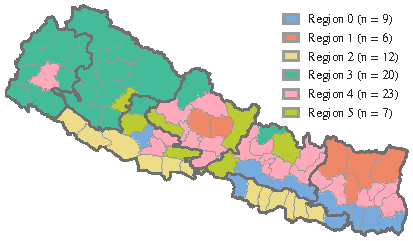
\includegraphics[width=\columnwidth]{fig-region-map.pdf}
\caption{The six K-means risk regions fitted on 2017 to 2022 profiles.}
\label{fig:regions}
\end{figure}

\subsection{Baseline Comparison and Main Result}
Tables~\ref{tab:main} and \ref{tab:mainops} give the main result over 2024 and 2025. District-by-month climatology already ranks well (PR-AUC 0.151, 95\% interval 0.128 to 0.176) because harm clusters in a few districts and months. Persistence is worse (0.102): only one in five damaging incidents (2020 to 2025) is known on the day it happens, and most harm does not repeat within three days. The Dahal and Hasegawa thresholds fire on 1.4\% of ERA5 district-days and catch 4\% of positives, so gauge thresholds do not transfer to a 0.25\textdegree{} grid. The refitted percentile threshold does no better than climatology (0.149).

Logistic regression, gradient boosting and the linear SVM reach 0.177 to 0.179, and their paired gains exclude zero (logistic regression +0.026, +0.005 to +0.049). The random forest, which the tuning rule had selected as best, scores 0.169, and its gain interval includes zero, as does the RBF SVM's (0.152). The three leading models differ by less than 0.002, so none is best. No interval is corrected for multiple comparisons, and the lower bounds are only 0.004 to 0.005, so the pattern across families matters more than any single model's gain. ROC-AUC rises from 0.664 for climatology to 0.69 to 0.71. The models separate from climatology mainly at recall below 0.5 (Fig.~\ref{fig:prcurves}(a)), the operating range of an alert system.

With calibrators fitted on out-of-fold scores of the training seasons, BSS is positive for all five models (0.006 to 0.019), with intervals above zero for all but the RBF SVM. Mean predicted probabilities of logistic regression and the random forest are 0.067 to 0.068 against an observed 0.085, because the test seasons had more harm than the training seasons (Fig.~\ref{fig:prcurves}(b)). At the 5\% budget (Fig.~\ref{fig:prcurves}(c)), logistic regression detects 14.3\% of positive district-days with a FAR of 0.76, against 11.8\% and 0.80 for climatology, and CSI rises from 0.080 to 0.099.

\begin{table}[t]
\caption{PR-AUC on 2024 to 2025 under the expanding window (per-season mean; 32,494 district-days, base rate 0.085) and paired difference from climatology (Clim.), with 95\% season-stratified weekly block-bootstrap intervals. Persist.: persistence; D\&H thr., ERA5 thr.: Dahal and Hasegawa and refitted thresholds; LR, RF, HGB, SVM-L, SVM-RBF: the five models; LR, set B: logistic regression with the perfect three-day rain forecast.}
\label{tab:main}
\centering
\scriptsize
\setlength{\tabcolsep}{4pt}
\begin{tabular}{lll}
\toprule
Model & PR-AUC [95\% CI] & $\Delta$ vs Clim. [95\% CI] \\
\midrule
\multicolumn{3}{l}{\textit{Baselines}} \\
Clim. & 0.151 [0.128, 0.176] &  \\
Persist. & 0.102 [0.083, 0.121] & $-$0.050 [$-$0.069, $-$0.034] \\
D\&H thr. & 0.091 [0.072, 0.110] & $-$0.060 [$-$0.083, $-$0.042] \\
ERA5 thr. & 0.149 [0.121, 0.173] & $-$0.003 [$-$0.030, +0.021] \\
\midrule\multicolumn{3}{l}{\textit{Models, set A (known at $t$)}} \\
LR & 0.177 [0.147, 0.210] & +0.026 [+0.005, +0.049] \\
RF & 0.169 [0.139, 0.196] & +0.017 [$-$0.005, +0.041] \\
HGB & 0.179 [0.147, 0.210] & +0.027 [+0.004, +0.051] \\
SVM-L & 0.177 [0.147, 0.209] & +0.026 [+0.005, +0.049] \\
SVM-RBF & 0.152 [0.129, 0.179] & +0.001 [$-$0.017, +0.020] \\
\midrule\multicolumn{3}{l}{\textit{Perfect-forecast ceiling}} \\
LR, set B & 0.207 [0.160, 0.257] & +0.056 [+0.016, +0.105] \\
\bottomrule
\end{tabular}

\end{table}

\begin{table}[t]
\caption{Probabilistic and operational skill on 2024 to 2025 under the expanding window: BSS of the out-of-fold calibrated probability with 95\% interval, ROC-AUC (ROC, per-season mean), and POD, FAR and CSI at the 5\% budget per season.}
\label{tab:mainops}
\centering
\scriptsize
\setlength{\tabcolsep}{4pt}
\begin{tabular}{llrrrr}
\toprule
Model & BSS [95\% CI] & ROC & POD & FAR & CSI \\
\midrule
Clim. &  & 0.664 & 0.118 & 0.800 & 0.080 \\
\midrule
LR & 0.017 [0.003, 0.031] & 0.708 & 0.143 & 0.757 & 0.099 \\
RF & 0.013 [0.001, 0.026] & 0.707 & 0.116 & 0.804 & 0.078 \\
HGB & 0.019 [0.004, 0.033] & 0.713 & 0.138 & 0.766 & 0.095 \\
SVM-L & 0.017 [0.004, 0.031] & 0.708 & 0.139 & 0.765 & 0.095 \\
SVM-RBF & 0.006 [$-$0.006, 0.019] & 0.694 & 0.110 & 0.813 & 0.074 \\
\midrule
LR, set B & 0.035 [0.007, 0.068] & 0.739 & 0.175 & 0.703 & 0.124 \\
\bottomrule
\end{tabular}

\end{table}

\begin{figure}[t]
\centering
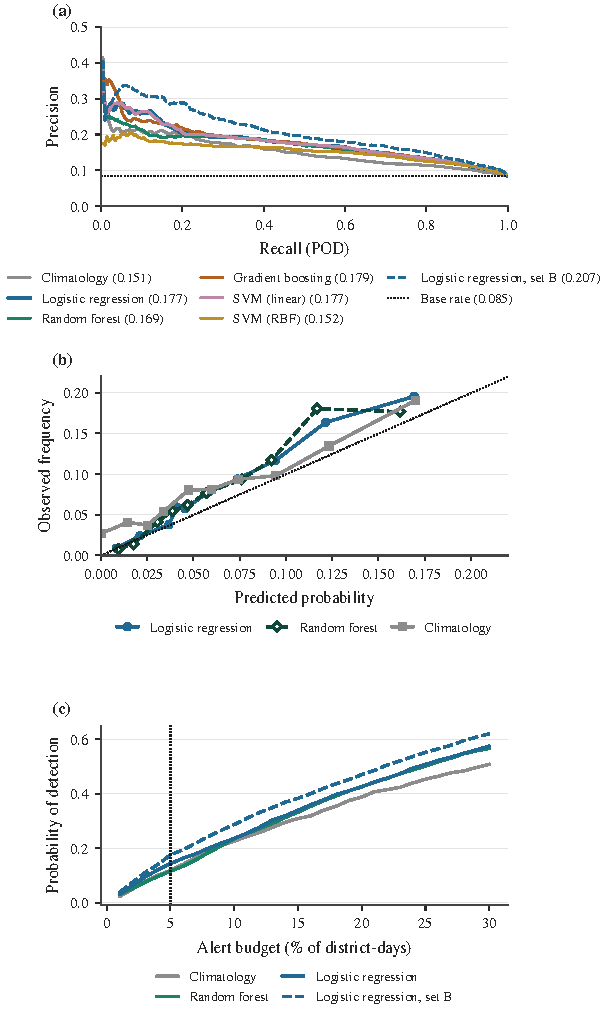
\includegraphics[width=\columnwidth]{fig-rolling-pr-reliability-budget.pdf}
\caption{Test 2024 to 2025 under the expanding window. (a) Precision-recall curves (per-season mean) of the set A models, climatology and logistic regression with set B. (b) Reliability of the out-of-fold calibrated logistic regression and random forest probabilities and of climatology. (c) POD against the per-season alert budget; dotted line: 5\%.}
\label{fig:prcurves}
\end{figure}

\subsection{Seasons and the 2026 Check}
All of the gain comes from 2024 (Table~\ref{tab:seasons}), the test year with most harm (base rate 0.090). In 2024, logistic regression reaches 0.217 against 0.164 for climatology (+0.052, +0.011 to +0.097), and the gain excludes zero for four of the five models. In 2025 every model is about level with climatology ($-0.014$ to $+0.007$). On the 2026 check (issue days to 16 August, base rate 0.058), climatology scores 0.102, up from 0.087 under the fixed split, where the models reached 0.100 to 0.108. No model's paired interval excludes zero; the best, the linear SVM, reaches 0.111 ($+0.009$, $-0.011$ to $+0.025$). BSS is positive for all five (0.005 to 0.013), but every interval includes zero. Starting training in 2020, the first season with prompt entry, shifts PR-AUC by at most 0.013 but changes which gains exclude zero: gradient boosting (0.187) and the random forest (0.180), not logistic regression (0.174).

\begin{table}[t]
\caption{PR-AUC per scored season under the expanding window, with the paired difference from climatology in brackets; $^{*}$: its 95\% interval excludes zero.}
\label{tab:seasons}
\centering
\scriptsize
\setlength{\tabcolsep}{4pt}
\begin{tabular}{llll}
\toprule
Model & 2024 & 2025 & 2026 check \\
\midrule
Fitted on & 2017--23 & 2017--24 & 2017--25 \\
Base rate & 0.090 & 0.079 & 0.058 \\
Clim. & 0.164 & 0.138 & 0.102 \\
\midrule
LR & 0.217 (+0.052)$^{*}$ & 0.138 ($-$0.001) & 0.110 (+0.008) \\
RF & 0.204 (+0.040)$^{*}$ & 0.133 ($-$0.005) & 0.104 (+0.002) \\
HGB & 0.212 (+0.048)$^{*}$ & 0.145 (+0.007) & 0.104 (+0.002) \\
SVM-L & 0.217 (+0.053)$^{*}$ & 0.138 (+0.000) & 0.111 (+0.009) \\
SVM-RBF & 0.181 (+0.016) & 0.124 ($-$0.014) & 0.093 ($-$0.009) \\
\midrule
LR, set B & 0.264 (+0.099)$^{*}$ & 0.151 (+0.013) & 0.116 (+0.014) \\
\bottomrule
\end{tabular}

\end{table}

\subsection{Ablations: Weather, Rules and Regions}
\label{sec:ablations}
On the fixed split, Table~\ref{tab:fsets} (appendix) separates the sources of skill, with paired intervals. Without any weather column (NOWX), logistic regression, gradient boosting and the linear SVM still reach 0.164 from season, terrain, history and recent incidents. The random forest without weather falls to climatology. Set A adds +0.011 to +0.022 to NOWX, with a paired interval that excludes zero only for the random forest. The perfect three-day rain forecast of set B adds another +0.034 to +0.054 for the four main families (0.211 to 0.220), with every interval above zero, and raises POD at the 5\% budget to 0.17. This gain is about three to four times the largest paired gap between the main families. On the rain-driven target, which leaves out lightning, climatology falls to 0.123 at a base rate of 0.055. Logistic regression reaches 0.177 with set A (paired gain +0.055, +0.019 to +0.096) and 0.229 with set B, a larger relative gain from rainfall information.

At each rule's own alert rate (Table~\ref{tab:rules}), logistic regression and the random forest detect more than all three rules. At the persistence rate they detect 20.6\% and 19.0\% against 17.2\%; at the rare Dahal and Hasegawa rate the margin is slight.

\begin{table}[t]
\caption{Rule baselines on test 2024 to 2025 at their own alert rate, against climatology, logistic regression and the random forest (set A, fixed split) re-thresholded to the same rate.}
\label{tab:rules}
\centering
\scriptsize
\setlength{\tabcolsep}{4pt}
\begin{tabular}{llrrrr}
\toprule
Rule (alert rate) & & Rule & Clim. & LR & RF \\
\midrule
Persist. (8.1\%) & POD & 0.172 & 0.181 & 0.206 & 0.190 \\
 & FAR & 0.820 & 0.811 & 0.785 & 0.801 \\
 & CSI & 0.096 & 0.102 & 0.118 & 0.108 \\
\addlinespace[2pt]
D\&H thr. (1.4\%) & POD & 0.041 & 0.031 & 0.047 & 0.044 \\
 & FAR & 0.755 & 0.812 & 0.716 & 0.737 \\
 & CSI & 0.036 & 0.028 & 0.042 & 0.039 \\
\addlinespace[2pt]
ERA5 thr. (21.3\%) & POD & 0.391 & 0.397 & 0.452 & 0.434 \\
 & FAR & 0.845 & 0.843 & 0.821 & 0.828 \\
 & CSI & 0.125 & 0.127 & 0.147 & 0.141 \\
\bottomrule
\end{tabular}

\end{table}

The regions do not help (Table~\ref{tab:regions}). For logistic regression every encoding is within $\pm 0.004$ of the model without region features, and the one-hot label is slightly worse. For the random forest, the posterior and distance encodings add +0.004 to +0.005 with intervals that include zero, while a plain district one-hot adds +0.005 (+0.002 to +0.008), as much as any region encoding. The pre-specified expectation that regions would help the linear model more than the trees is not supported.

\begin{table}[t]
\caption{Objective 3: PR-AUC on test with the four location encodings added to set A (fixed split), and paired differences against the same model without them (RF: random forest; LR: logistic regression).}
\label{tab:regions}
\centering
\scriptsize
\begin{tabular}{llll}
\toprule
Model & Encoding & PR-AUC & $\Delta$ vs none [95\% CI] \\
\midrule
RF & none (set A) & 0.165 &  \\
 & + K-means label & 0.166 & +0.001 [$-$0.002, +0.004] \\
 & + GMM posteriors & 0.170 & +0.005 [$-$0.001, +0.011] \\
 & + centroid distances & 0.169 & +0.004 [$-$0.002, +0.011] \\
 & + district one-hot & 0.170 & +0.005 [+0.002, +0.008] \\
\addlinespace[2pt]
LR & none (set A) & 0.177 &  \\
 & + K-means label & 0.174 & $-$0.004 [$-$0.008, +0.001] \\
 & + GMM posteriors & 0.176 & $-$0.002 [$-$0.006, +0.002] \\
 & + centroid distances & 0.178 & +0.000 [$-$0.005, +0.005] \\
 & + district one-hot & 0.175 & $-$0.003 [$-$0.009, +0.003] \\
\addlinespace[2pt]
\bottomrule
\end{tabular}

\end{table}

\subsection{Where the Forecast Fails and What Drives It}
The forecast is most useful for rain-driven hazards and in mid-season, and least for lightning. Table~\ref{tab:errors} and Fig.~\ref{fig:errors} (appendix) break the fixed-split random forest down by region, belt, hazard and month. By region, the gain over climatology is largest in the central and western Terai (region 2: 0.206 against 0.166) and the central Hill belt (region 4: 0.139 against 0.109). The six wet eastern districts of region 1 score below climatology (0.151 against 0.173) and receive few alerts (POD 0.04). A national budget also spreads alerts unevenly: it alerts 9\% of rows in regions 0 and 5 but about 3\% in region 3 and 2\% in the Mountain belt, which argues for regional budgets.

By hazard, the all-hazard model ranks floods, heavy rainfall and landslides better than climatology and lightning worse (0.038 against 0.043). The perfect-forecast ceiling raises the first three by 60 to 120\% but leaves lightning almost unchanged (0.045), consistent with its convective mechanism. By month, detection peaks in July (POD 0.22) and is weakest in April and May (0.03 to 0.06), when lightning dominates and the model issues almost no alerts. In August the model under-performs climatology (0.164 against 0.191), as positives spread over many districts after a wet July.

\begin{table}[t]
\caption{Random forest (set A, fixed split) on test 2024 to 2025 by region, belt and hazard, with POD at the national 5\% budget. Hazard rows score the all-hazard model against each hazard's own label.}
\label{tab:errors}
\centering
\scriptsize
\begin{tabular}{lrrrrr}
\toprule
Stratum & Pos. & Base & Clim. & RF & POD \\
\midrule
Region 0 & 350 & 0.092 & 0.145 & 0.162 & 0.160 \\
Region 1 & 271 & 0.107 & 0.173 & 0.151 & 0.037 \\
Region 2 & 353 & 0.070 & 0.166 & 0.206 & 0.218 \\
Region 3 & 756 & 0.090 & 0.183 & 0.196 & 0.093 \\
Region 4 & 735 & 0.076 & 0.109 & 0.139 & 0.095 \\
Region 5 & 284 & 0.096 & 0.155 & 0.154 & 0.151 \\
\addlinespace[2pt]
Terai & 590 & 0.067 & 0.123 & 0.167 & 0.185 \\
Hill & 1500 & 0.096 & 0.146 & 0.163 & 0.119 \\
Mountain & 659 & 0.082 & 0.162 & 0.175 & 0.058 \\
\addlinespace[2pt]
Flood (own label) & 467 & 0.014 & 0.024 & 0.041 & 0.161 \\
Landslide (own label) & 827 & 0.025 & 0.051 & 0.062 & 0.143 \\
Heavy rainfall (own label) & 725 & 0.022 & 0.047 & 0.067 & 0.167 \\
Lightning (own label) & 1054 & 0.032 & 0.043 & 0.038 & 0.052 \\
\bottomrule
\end{tabular}

\end{table}

No single feature dominates the random forest (Fig.~\ref{fig:shap}). By mean absolute SHAP value the 3-day rain percentile (0.025), rain on day $t$ (0.023) and the district history rate (0.020) lead. High rain percentiles, high history rates and mid-season days push the score up. High elevation pushes it down. So do high 30-day totals, because the wettest late-season weeks fall after the damage peak. Permutation importance agrees on the rain features for the random forest but, for logistic regression, ranks season far higher (day-of-year sine 0.035). The linear model relies on a smooth seasonal curve, while the forest uses history and rain interactions.

\begin{figure}[t]
\centering
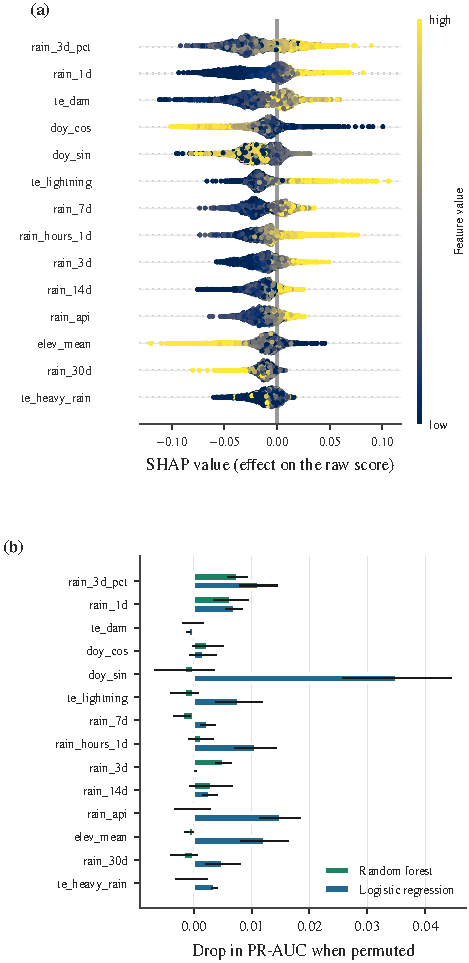
\includegraphics[width=\columnwidth]{fig-shap-permutation.pdf}
\caption{(a) SHAP summary for the random forest (set A, fixed split) on a stratified sample of 4,000 test rows. (b) Permutation importance (drop in PR-AUC) for the random forest and logistic regression on the same rows.}
\label{fig:shap}
\end{figure}

\subsection{Case Study: 26 to 28 September 2024}
\label{sec:case}
From 26 to 28 September 2024 a late-monsoon system stalled over central and eastern Nepal and brought record three-day rain \cite{Lamichhane2025}. Over those days BIPAD recorded 232 damaging incidents in 42 of the 77 districts, mostly landslides and floods, the worst event in the record. Fig.~\ref{fig:case} shows the forecast issued at the end of 25 September. With set A, the random forest ranks the districts no better than climatology (PR-AUC 0.579 against 0.595). Six of its top 10 and 9 of its top 20 districts were hit, against 4 and 11 for climatology. Its probabilities stay below 0.09 everywhere, because ERA5 rain up to 25 September had not yet shown the extreme totals of 27 and 28 September. The set B version, which sees that rain, raises the whole central and eastern belt (PR-AUC 0.771; 8 of the top 10 and 15 of the top 20 hit) and leaves the dry west low. Set B's gain over set A came from knowing the coming rain.

\begin{figure}[!t]
\centering
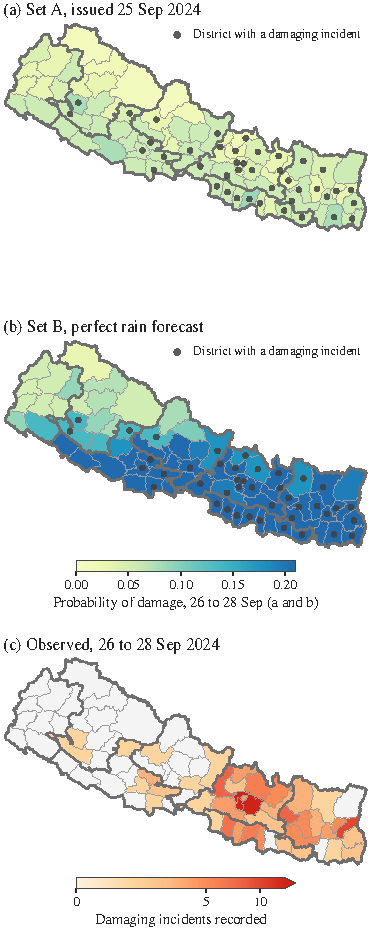
\includegraphics[width=\columnwidth,height=5.3in,keepaspectratio]{fig-case-study-2024-09.pdf}
\caption{Forecast issued at the end of 25 September 2024. (a) Random forest (fixed split) probability with set A; (b) with set B (perfect forecast). Dots mark districts that recorded damaging incidents on 26 to 28 September; (a) and (b) share one colour scale. (c) Damaging incidents per district on those days (scale capped at the 95th percentile).}
\label{fig:case}
\end{figure}

\section{Discussion and Conclusions}
\subsection{Summary and Comparison with the Literature}
Objective 1 produced six moderately stable, interpretable monsoon risk regions that differ from the belts and the provinces. Objective 2 produced a district-day harm forecast with small but measurable ranking skill, concentrated in one of two test seasons. Objective 3 found that the regions add nothing to the models. Skill numbers are not directly comparable across studies because targets and base rates differ, but the pattern is. Stanley et al. about doubled the hit rate of a heuristic landslide nowcast \cite{Stanley2021}, Iglesias et al. beat the official warning \cite{Iglesias2024}, and Morales et al. found that the choice of model matters little \cite{Morales2026}. In this study most of the predictable signal is spatial and seasonal, and the daily increment from weather is the hard part. The null result for regions is largely expected by construction, because the pooled model already encodes district-by-month history. It is consistent with Piernik and Morzy's finding that cluster features help only in some settings \cite{Piernik2021}, but it does not test the pooled-against-regional comparison of hydrology \cite{Kratzert2019,Fang2022}.

\subsection{Interpretation}
First, the floor is high and the ceiling low. Day-$t$ reanalysis rain adds only 0.01 to 0.02 to the no-weather floor of 0.164 (fixed split), while a perfect three-day rain forecast adds 0.03 to 0.05 more, so the coming rain matters more than the rain already observed. Second, lightning weakens the all-hazard target. It is the only hazard in 36\% of positives, peaks before the monsoon and is weakly tied to daily rain, so the model learns two hazard types at once. Third, calibration follows the base rates of its fitting seasons: fitted on 2023, the quietest season, it left BSS near zero or negative (fixed split); fitted on several seasons, it gives positive BSS but still under-predicts the wetter test years, so an operational system would recalibrate each season \cite{Hamill2006}.

\subsection{Trends in the Field and Their Limits Here}
Hazard forecasting is moving from rainfall thresholds to learned models \cite{Stanley2021,Doerksen2023,Iglesias2024}. The results favour better rain input, although reanalysis rain over the Himalaya is itself uncertain \cite{Chen2021}. They give no reason for more model capacity: the four families are close, and a harm label that reflects reporting as much as weather \cite{Gall2009,Jones2022} caps what any model can extract. For a record like BIPAD, label quality, exposure data and time-ordered evaluation of triggers \cite{Kapoor2023,Potter2025} are likely to return more than model complexity.

\subsection{Practical Implications}
Set A is a hindcast: ERA5 arrives about five days late, so none of its rain is available at issue time. A FAR of 0.76 is also too high for a cash-release trigger. The output suits a daily readiness and prioritisation ranking of districts under a fixed alert budget, for District Disaster Management Committees and local governments alongside the heavy-rain and flood warnings of the Department of Hydrology and Meteorology. At about four alerts a day it detects about 14\% of damaging district-days with three false alarms per hit, against about 12\% and four for climatology.

\subsection{Social, Ethical, Legal and Professional Considerations}
\label{sec:ethics}
A missed alert and a false alarm have different costs: the first can cost lives, the second credibility and, under anticipatory action, money released for nothing. The 5\% budget used here favours detection, and a deployed system should set its budget with the agencies that act on it. The model learns from what BIPAD records. Loss records and landslide inventories tend to miss remote areas \cite{Gall2009,Harvey2024}, and Nepal's recorded lightning deaths rose with internet access \cite{Adhikari2021}; this was not tested for BIPAD. A district with no record is not necessarily safe. Districts with weaker reporting would receive lower scores, so an alert system built on these scores could steer attention away from those who need it most. BIPAD is public with no stated licence; Open-Meteo's ERA5 data are CC BY 4.0, the Copernicus DEM has its own licence and COD-AB is CC BY-IGO. Loss counts are discarded after labelling, so no person is identifiable and no incident-level loss value is published. NDRRMA holds the record under the Disaster Risk Reduction and Management Act 2017, which created it and charged it with running a national disaster information system \cite{DRRMAct2017}. The model is a research prototype, unvalidated for operational warning. Following the ACM Code of Ethics \cite{ACM2018}, the study puts public benefit first and reports its limits and risks.

\subsection{Limitations and Future Work}
The evidence of skill rests on one season, 2024, so more test seasons are needed. Hyperparameters were tuned once, on 2017 to 2022. The expanding window replaced the fixed split after both had scored the test seasons; under the fixed split, three models beat climatology in 2026. The label is a reporting record with two entry periods and growing coverage; the damaging filter and the year controls reduce but do not remove the effect. Set A uses the ERA5 analysis of day $t$, so its skill is an upper bound on what the same features would give operationally; set B is a ceiling by design. One reanalysis point per district smooths orographic rain, and the free archive has no convective variables, which limits lightning. Slope from a 30 m DEM and the susceptibility layer of Kincey et al. \cite{Kincey2024,Kincey2023Data}, planned in the proposal, were not used; terrain came from ward-centroid elevation. Floods from suspected landslide blockages, such as the Gorkha flood, or from glacier failures can strike on dry days and are outside the model's scope. Future work should use archived operational forecasts at one to three day leads and add lightning observations or convective indices. It should also move to municipality units where the ward link allows, and add exposure so that the target can be weighted by people at risk.

\subsection{Conclusion}
This study built a district-day harm dataset for Nepal's four main monsoon hazards from open data and tested whether machine learning can forecast when and where harm will occur. Under an expanding window, logistic regression, gradient boosting and the linear SVM beat climatology by about 0.026 in PR-AUC, with lower bounds near zero, while the pre-specified random forest did not. The gain came from 2024; in 2025 and the 2026 check no model clearly beat climatology. Knowing the coming rain would help more than changing the model, so better rain forecasts matter most. The risk regions, though moderately stable and interpretable, added nothing to a pooled model on the fixed split. The code and frozen data (Appendix~\ref{app:run}) reproduce every number.

\appendices
\section{Code and Data Availability}
\label{app:run}
The code is available at \codeurl{}, with a video walkthrough: \url{https://youtu.be/Js4m7qHRn3s}. The frozen inputs (BIPAD snapshot of 19 September 2026, the frozen BIPAD geography, the ERA5 archive and the terrain and boundary files) are included with their \path{.meta.json} provenance, so the commands below run offline.

\subsection{Reproducing the Results}
From a clone of the repository, the commands below install the locked environment, rebuild the panel and feature matrix, run the checks, execute notebooks 01 to 05 in order, run the expanding-window evaluation and regenerate the main-result figure and the tables. Notebooks 04 and 05 train and analyse the fixed-split model of the diagnostic analyses; notebook 04 saves the models that notebook 05 reads, since trained models are not shipped. The notebooks take about 27 minutes on the M4 laptop (Table~\ref{tab:runtimes}) and \path{src.rolling} about 18 minutes; Fig.~\ref{fig:notebook} shows the main-result cell of the executed notebook 04.

{\scriptsize
\begin{verbatim}
# install the locked environment
$ uv sync
# build the district-day panel from frozen inputs
$ uv run python -m src.panel
# build the feature matrix
$ uv run python -m src.freeze
# run the leakage checks
$ uv run python -m src.checks
# run notebooks 01 to 05 (fixed-split analyses)
$ uv run jupyter nbconvert --to notebook --execute \
    --inplace notebooks/0*.ipynb
# expanding-window evaluation (main results)
$ uv run python -m src.rolling
# rule baselines under the expanding window
$ uv run python -m src.rolling baselines
# main-result figure
$ uv run python -m src.plotting
# all paper tables
$ uv run python -m src.tables
\end{verbatim}
}

\begin{figure}[!t]
\centering
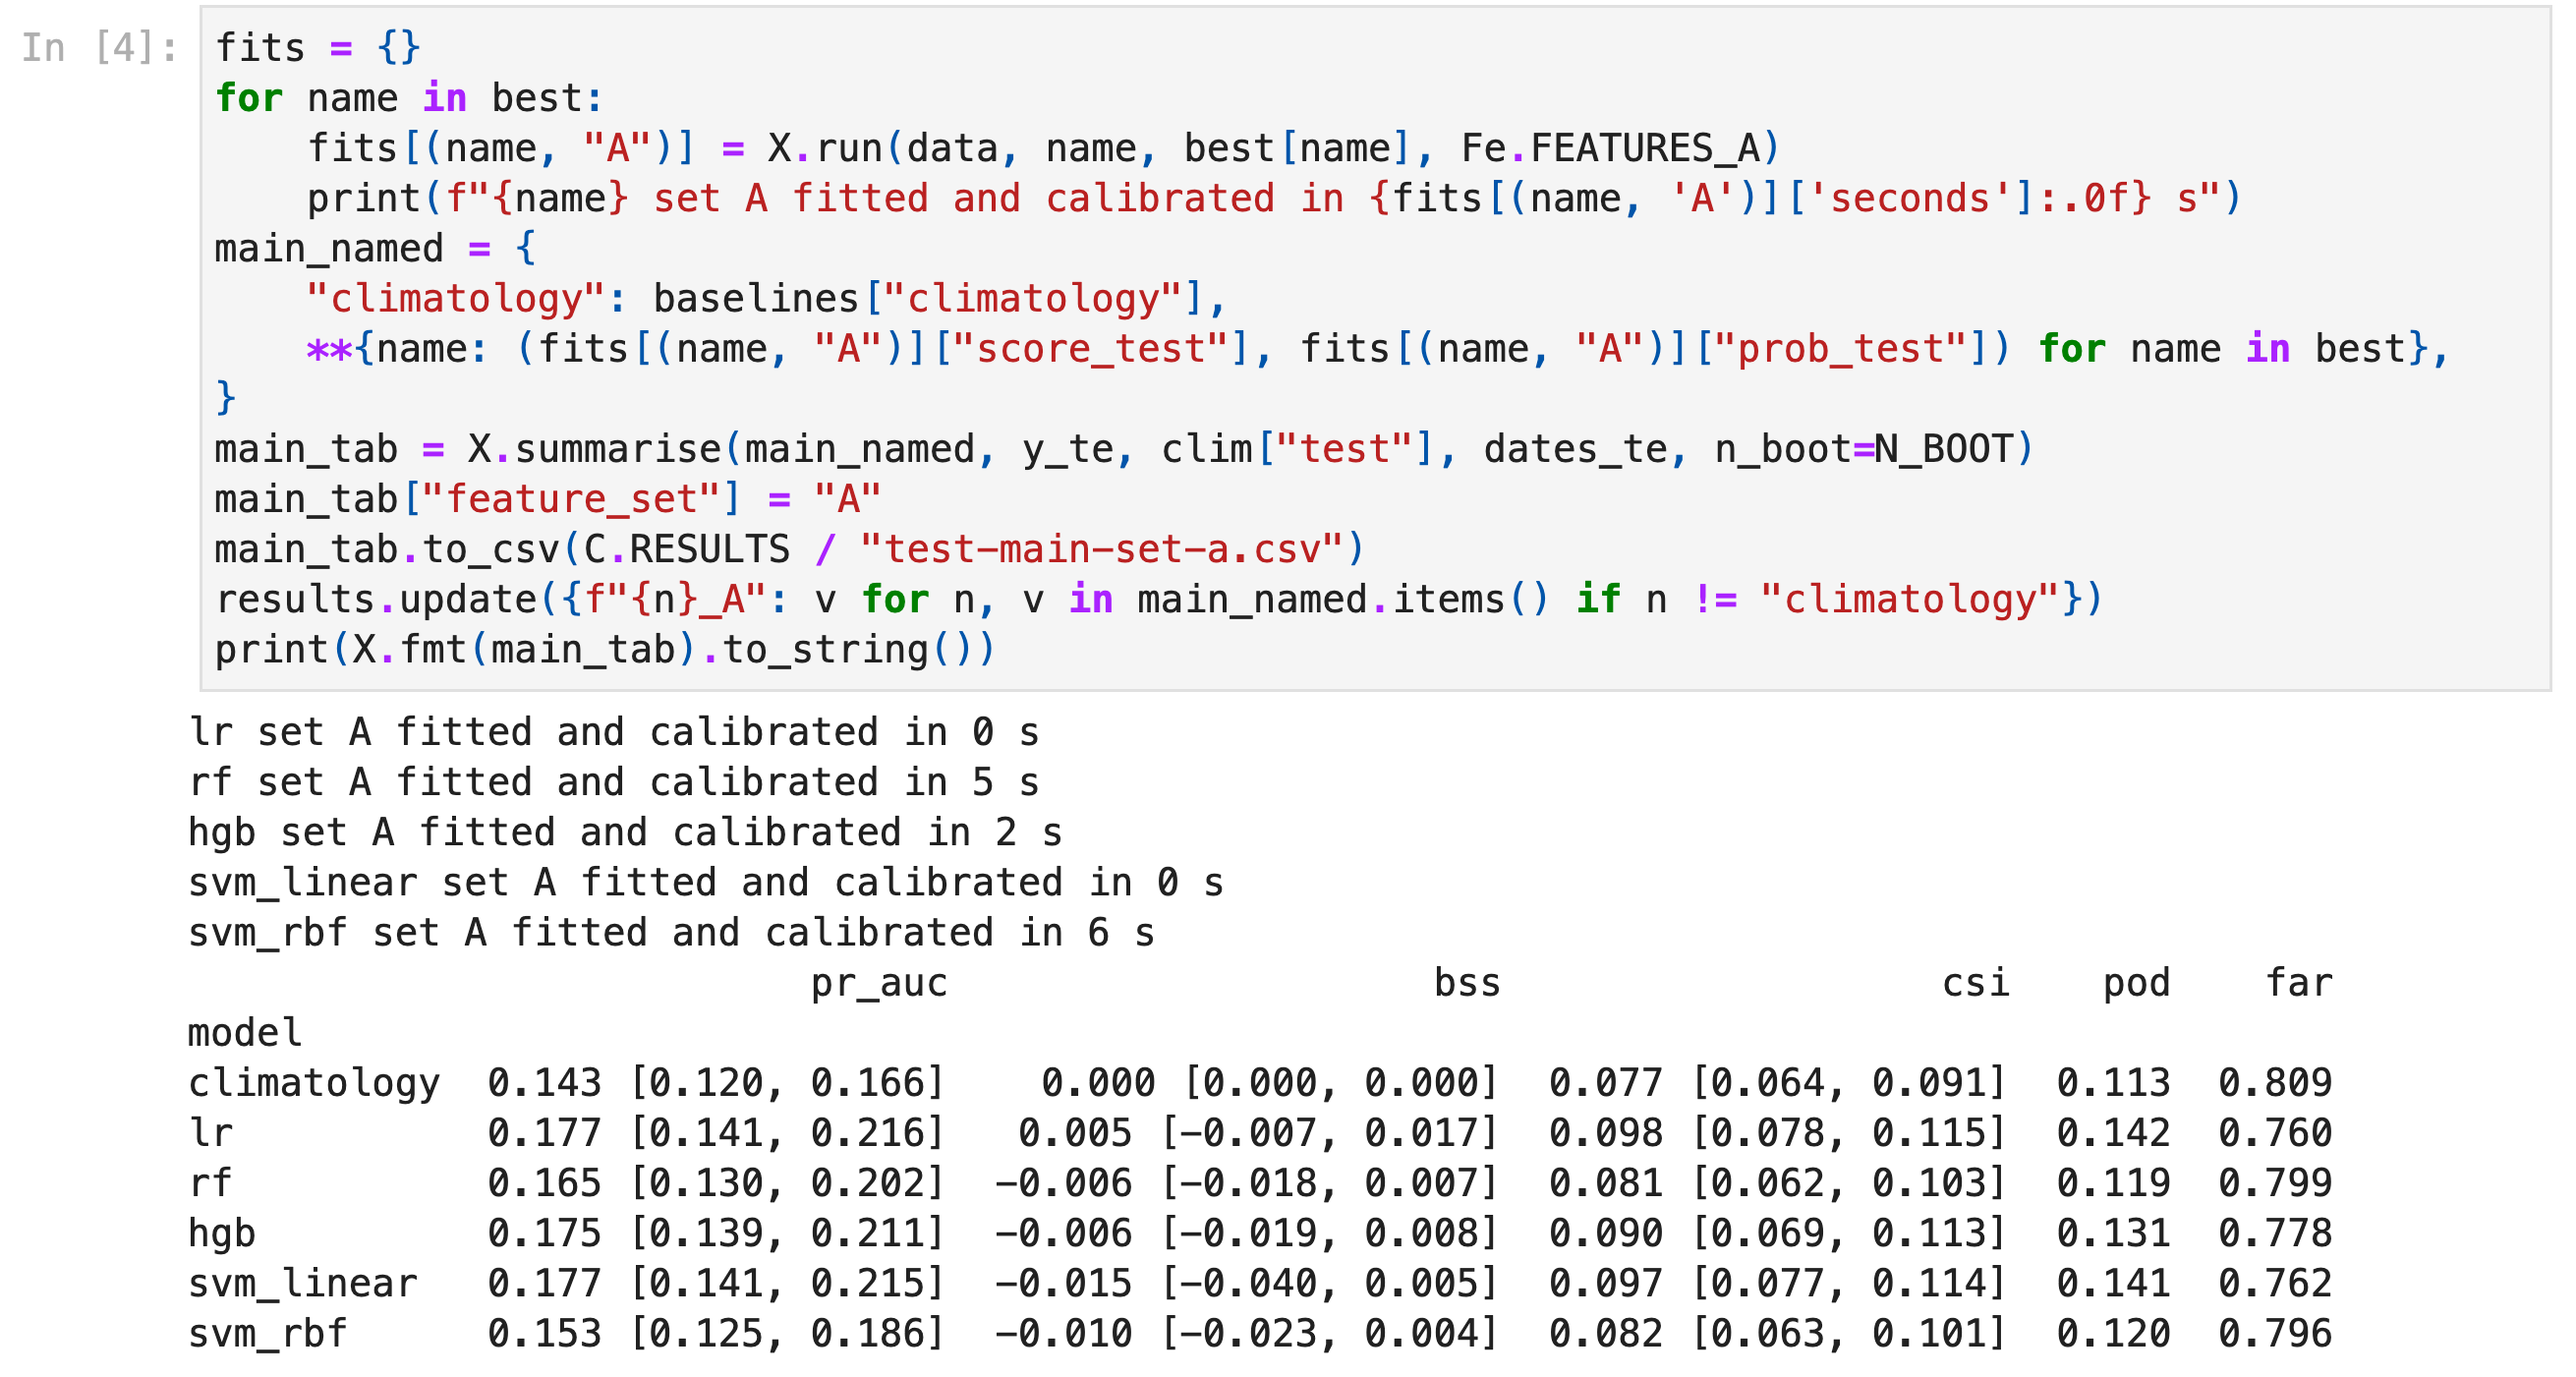
\includegraphics[width=\columnwidth]{fig-notebook-screenshot.png}
\caption{Main-result cell of the executed notebook 04: the fixed-split model used for the diagnostic analyses, not the expanding-window results of Table~\ref{tab:main}.}
\label{fig:notebook}
\end{figure}

\subsection{Environment and Run Times}
All runs were on an Apple M4 laptop (24 GB) under macOS 26.3 with Python 3.12.12, pandas 3.0.6, numpy 2.5.3, scikit-learn 1.9.1, matplotlib 3.11.2, seaborn 0.13.2, geopandas 1.2.0, shap 0.53.0 and pyarrow 26.0.0, pinned exactly in \path{uv.lock} (and in \path{pyproject.toml}, where geopandas and seaborn have lower bounds only) and exported to \path{requirements.txt}. The five notebooks were executed top to bottom from a clean kernel with \texttt{jupyter nbconvert}. The final clean run took 27.4 minutes in total, of which notebook 04 (tuning and bootstraps) took 16.3 minutes. Every random element uses seed 42, and the tables reproduce exactly across runs. Table~\ref{tab:runtimes} lists the run time of each notebook. The output of \path{src.checks} follows. The executed notebooks keep their cell outputs.

\begin{table}[!t]
\caption{Clean run of the five notebooks.}
\label{tab:runtimes}
\centering
\scriptsize
\begin{tabular}{lrr}
\toprule
Notebook & Exit & Seconds \\
\midrule
01-data-preparation & 0 & 9 \\
02-exploratory-analysis & 0 & 17 \\
03-clustering-risk-regions & 0 & 11 \\
04-classification & 0 & 980 \\
05-evaluation-and-interpretation & 0 & 628 \\
\bottomrule
\end{tabular}

\end{table}

{\scriptsize
\begin{verbatim}
$ uv run python -m src.checks
panel (156849, 20), incidents (16790, 8), terrain (77, 5)
ok  panel reproduces the reference numbers
ok  feature lists: no loss_*/target columns,
    set A has no future_*, NOWX has no weather
ok  no loss_* columns in panel or incidents table
ok  set A unchanged when the future is scrambled
  259 recent-incident window counts recomputed by hand
ok  entry-lag rule: known-at-t counts, synthetic
    pre-2020 lags
ok  percentiles and target encoding use training
    seasons only
ok  leave-one-season-out target encoding for training rows
ok  persistence baseline uses known-at-t incidents only
  real ERA5 coverage of panel rows: 100.00%
  real ERA5 rain features on cached seasons:
    (171710, 14), mean 7-day rain 71.2 mm
ok  real-weather smoke test
all checks passed
\end{verbatim}
}

\subsection{Features and Hyperparameters}
Table~\ref{tab:features} defines every feature in sets A and B, and Table~\ref{tab:hyper} gives the hyperparameter grids, the settings chosen by leave-one-season-out tuning and their mean fold PR-AUC. Table~\ref{tab:folds} shows each chosen setting fold by fold. The spread across held-out seasons (SD about 0.03) is about twice the gap between the four main families, and fold skill broadly follows the season's base rate. For this reason the families are treated as close. The linear models are insensitive to $C$ across the grid, and the random forest, gradient boosting and RBF choices sit at grid edges, so the comparison holds within the grids searched. Table~\ref{tab:counts} turns the 5\% budget on the test seasons (1,624 alerts, expanding window) into counts.
\begin{table}[!t]
\caption{Feature sets. Set A is the first five groups, set B adds the last group, and NOWX drops the rain group.}
\label{tab:features}
\centering
\scriptsize
\begin{tabular}{p{0.9cm}p{3.0cm}p{3.55cm}}
\toprule
Group & Feature & Definition \\
\midrule
Rain (A) & \texttt{rain\_1d} & ERA5 precipitation on day $t$ (mm) \\
 & \texttt{rain\_3d} & Sum over $t-2$ to $t$ (mm) \\
 & \texttt{rain\_7d} & Sum over 7 days (mm) \\
 & \texttt{rain\_14d} & Sum over 14 days (mm) \\
 & \texttt{rain\_30d} & Sum over 30 days (mm) \\
 & \texttt{rain\_api} & Antecedent precipitation index, decay 0.9 \\
 & \texttt{rain\_hours\_1d} & Hours with precipitation on day $t$ \\
 & \texttt{tmax\_1d} & Maximum 2 m temperature on day $t$ (\textdegree C) \\
 & \texttt{rain\_3d\_pct} & Percentile of the 3-day sum in the district's 2017 to 2022 distribution \\
Season & \texttt{doy\_sin} & Day of year, sine \\
 & \texttt{doy\_cos} & Day of year, cosine \\
 & \texttt{month} & Calendar month \\
Terrain & \texttt{elev\_mean} & Mean ward elevation (m) \\
 & \texttt{elev\_relief} & Ward elevation range (m) \\
 & \texttt{share\_above\_1000m} & Share of wards above 1,000 m \\
 & \texttt{share\_above\_3000m} & Share of wards above 3,000 m \\
Recent incidents & \texttt{recent\_dam\_3d} & Damaging incidents known at $t$, dated $t-3$ to $t$ \\
 & \texttt{recent\_dam\_7d} & Same, $t-7$ to $t$ \\
 & \texttt{nbr\_recent\_dam\_3d} & Same as recent\_dam\_3d, summed over neighbouring districts \\
 & \texttt{nbr\_recent\_dam\_7d} & Same, 7 days \\
 & \texttt{recent\_flood\_7d} & Flood incidents, 7 days \\
 & \texttt{recent\_landslide\_7d} & Landslide incidents, 7 days \\
 & \texttt{recent\_heavy\_rain\_7d} & Heavy-rainfall incidents, 7 days \\
 & \texttt{recent\_lightning\_7d} & Lightning incidents, 7 days \\
History & \texttt{te\_dam} & District $\times$ month rate of damaging days (shrunk, leave-one-season-out) \\
 & \texttt{te\_flood} & Same, flood \\
 & \texttt{te\_landslide} & Same, landslide \\
 & \texttt{te\_heavy\_rain} & Same, heavy rainfall \\
 & \texttt{te\_lightning} & Same, lightning \\
Future rain (B) & \texttt{future\_rain\_3d} & Observed ERA5 rain, $t+1$ to $t+3$ (mm); set B only \\
 & \texttt{future\_rain\_max\_1d} & Maximum daily rain, $t+1$ to $t+3$; set B only \\
 & \texttt{future\_rain\_hours\_3d} & Rain hours, $t+1$ to $t+3$; set B only \\
\bottomrule
\end{tabular}

\end{table}

\begin{table}[!t]
\caption{Hyperparameter grids, chosen settings and mean leave-one-season-out PR-AUC (2017 to 2022, set A).}
\label{tab:hyper}
\centering
\scriptsize
\begin{tabular}{p{0.8cm}p{3.0cm}p{1.95cm}r}
\toprule
Model & Grid and fixed settings & Chosen & Fold PR-AUC \\
\midrule
LR & C $\in$ \{0.01, 0.1, 1.0\};\newline L2, class weight balanced, standardised inputs & C = 0.01 & 0.136 \\
RF & min\_samples\_leaf $\in$ \{20, 100\};\newline max\_features $\in$ \{sqrt, 0.5\};\newline 300 trees, class weight balanced-subsample & min\_samples\_leaf = 20, max\_features = sqrt & 0.150 \\
HGB & learning\_rate $\in$ \{0.03, 0.1\};\newline max\_leaf\_nodes $\in$ \{15, 31\};\newline 300 iterations, min leaf 50, L2 1.0, class weight balanced & learning\_rate = 0.03, max\_leaf\_nodes = 15 & 0.148 \\
SVM-L & C $\in$ \{0.001, 0.01, 0.1\};\newline LinearSVC, class weight balanced, standardised & C = 0.1 & 0.135 \\
SVM-RBF & C $\in$ \{0.3, 1.0\};\newline gamma $\in$ \{scale\};\newline RBF, $\gamma$ = scale, 12,000-row stratified subsample & C = 0.3, gamma = scale & 0.118 \\
\bottomrule
\end{tabular}

\end{table}

\begin{table}[!t]
\caption{Leave-one-season-out PR-AUC of each chosen setting by held-out season (set A), with the season's positive rate.}
\label{tab:folds}
\centering
\scriptsize
\setlength{\tabcolsep}{3.5pt}
\begin{tabular}{lrrrrrr}
\toprule
Held out & Base (\%) & LR & RF & HGB & SVM-L & SVM-RBF \\
\midrule
2017 & 5.9 & 0.144 & 0.151 & 0.160 & 0.139 & 0.124 \\
2018 & 6.8 & 0.119 & 0.119 & 0.128 & 0.120 & 0.120 \\
2019 & 6.5 & 0.169 & 0.187 & 0.174 & 0.167 & 0.120 \\
2020 & 8.2 & 0.173 & 0.193 & 0.194 & 0.173 & 0.137 \\
2021 & 7.1 & 0.128 & 0.139 & 0.140 & 0.126 & 0.106 \\
2022 & 5.4 & 0.086 & 0.111 & 0.089 & 0.085 & 0.098 \\
\midrule
Mean & & 0.136 & 0.150 & 0.148 & 0.135 & 0.118 \\
SD & & 0.033 & 0.034 & 0.037 & 0.033 & 0.014 \\
Min & & 0.086 & 0.111 & 0.089 & 0.085 & 0.098 \\
Max & & 0.173 & 0.193 & 0.194 & 0.173 & 0.137 \\
\bottomrule
\end{tabular}

\end{table}

\begin{table}[!t]
\caption{Alert outcomes at the 5\% budget on test 2024 to 2025 under the expanding window (1,624 alerts, 2,749 positives).}
\label{tab:counts}
\centering
\scriptsize
\begin{tabular}{lrrrr}
\toprule
Model & Hits & False alarms & Misses & Correct neg. \\
\midrule
Clim. & 325 & 1,299 & 2,424 & 28,446 \\
LR & 394 & 1,230 & 2,355 & 28,515 \\
RF & 318 & 1,306 & 2,431 & 28,439 \\
HGB & 380 & 1,244 & 2,369 & 28,501 \\
SVM-L & 381 & 1,243 & 2,368 & 28,502 \\
SVM-RBF & 303 & 1,321 & 2,446 & 28,424 \\
LR, set B & 482 & 1,142 & 2,267 & 28,603 \\
\bottomrule
\end{tabular}

\end{table}

\subsection{Leakage Audit}
\path{src/checks.py} runs eight groups of assertions. Its output is listed above. The checks are: (1) the panel reproduces the reference numbers (146,223 rows, 6.81\% positive, rates of 6.65, 4.44 and 8.46\% in 2017 to 2022, 2023 and 2024 to 2025, 2026 check 10,626 rows at 5.78\%); (2) no \path{loss_*}, target, same-day outcome or identifier column is a feature, set A has no \path{future_*} column and NOWX has no weather column; (3) set A is unchanged when all weather after an arbitrary cutoff is scrambled and all incidents not yet entered at the cutoff are removed; (4) recent-incident counts never include an incident before its entry day, pre-2020 synthetic lags match the 2020 to 2025 distribution, and 259 window counts recomputed by hand agree; (5) rain percentiles and history rates do not change when test-season data are altered; (6) a training row's history encoding does not change when its own season's outcomes are altered, and test rows use all six training seasons; (7) the persistence baseline uses known-at-$t$ incidents only; (8) with the full ERA5 archive no feature is missing. Checks (4) to (6) test the fixed-split build; \path{src.rolling} first asserts that its per-season rebuild reproduces that build exactly, then refits every fitted quantity per scored season.

Three residual points are stated for completeness. Within the tuning folds, the rain percentiles and the training rows' history encoding were fitted once on all six training seasons, so a held-out tuning season is not fully unseen; this can flatter fold scores but cannot reach the test seasons. The expanding-window calibration folds rebuild their features and do not share this. The fixed-split model's synthetic entry lags are drawn from the entry-date metadata of 2020 to 2025 incidents, test seasons included, though no label enters them; in the expanding window each scored season draws them from 2020 up to the season before it. Year is not a feature of any model. The year-only control has no district term, so its position below climatology says nothing about leakage. The proper check adds year to a control on the shrunk district-by-month history rate and month: test PR-AUC moves from 0.136 to 0.138 (paired difference +0.002, +0.000 to +0.004), and the fitted year coefficient is close to zero.

\subsection{Additional Figures and Tables}
Figs.~\ref{fig:seasonality} to \ref{fig:errors} and Table~\ref{tab:fsets} support the exploratory findings, the risk regions and the ablations reported in Section~\ref{sec:results}.
\begin{figure}[!t]
\centering
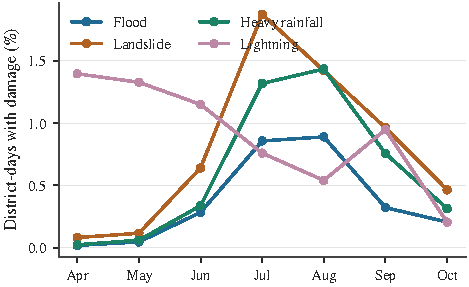
\includegraphics[width=\columnwidth]{fig-seasonality-by-hazard.pdf}
\caption{Share of district-days with a damaging incident of each hazard by month, 2017 to 2025.}
\label{fig:seasonality}
\end{figure}

\begin{figure}[!t]
\centering
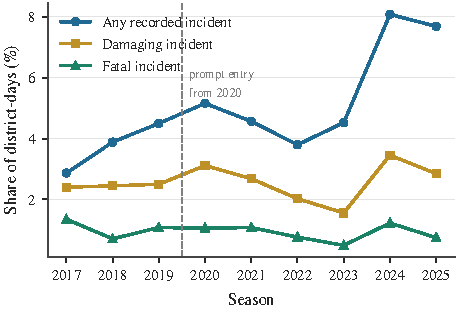
\includegraphics[width=\columnwidth]{fig-damaging-days-per-year.pdf}
\caption{Share of district-days per season with any recorded incident, a damaging incident and a fatal incident.}
\label{fig:peryear}
\end{figure}

\begin{figure}[!t]
\centering
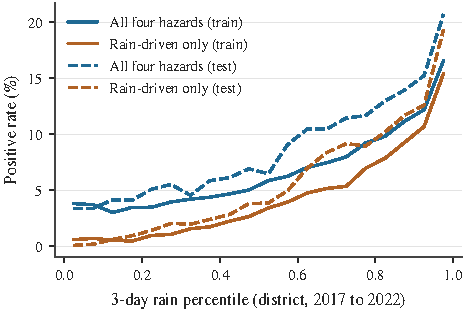
\includegraphics[width=\columnwidth]{fig-rain-percentile-vs-rate.pdf}
\caption{Positive rate against the 3-day rain percentile (district, 2017 to 2022) for the all-hazard and rain-driven targets, in training and test seasons.}
\label{fig:rainpct}
\end{figure}

\begin{figure}[!t]
\centering
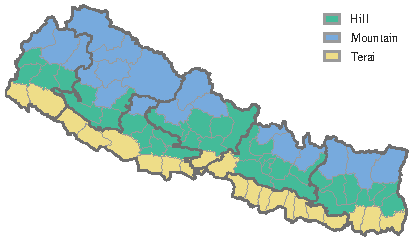
\includegraphics[width=\columnwidth]{fig-district-rate-map-b.pdf}
\caption{Ecological belt proxy derived from ward elevations (Section~\ref{sec:area}).}
\label{fig:belts}
\end{figure}

\begin{figure}[!t]
\centering
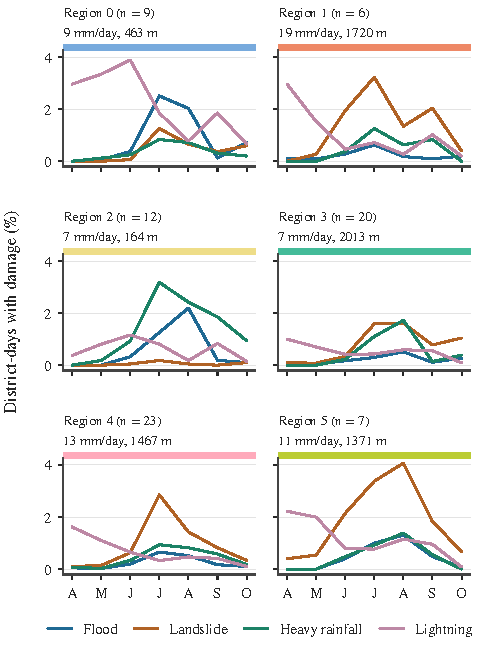
\includegraphics[width=\columnwidth]{fig-region-profiles.pdf}
\caption{Monthly rate of damaging days per hazard in each region, 2017 to 2022, with the region's size, mean daily rain and mean elevation.}
\label{fig:profiles}
\end{figure}

% Fig. of validity indices against k, left out because Table~\ref{tab:cluster} gives the same values;
% restore this block if space allows.
% \begin{figure}[!t]
% \centering
% 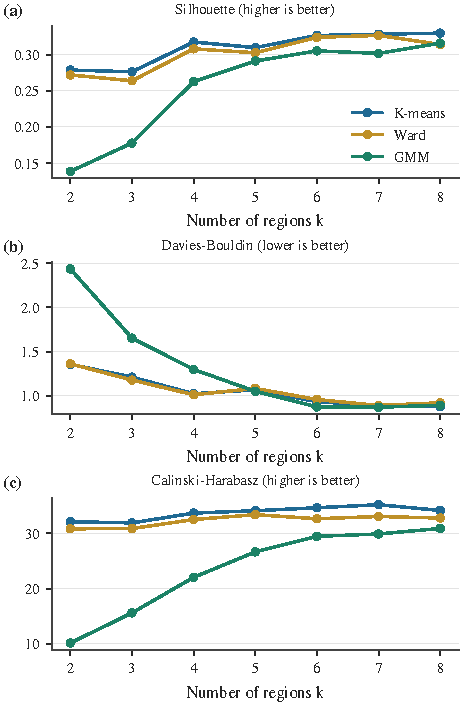
\includegraphics[width=\columnwidth]{fig-cluster-validity.pdf}
% \caption{Validity indices against $k$ for the three clusterers in the four-component space.}
% \label{fig:validity}
% \end{figure}

\begin{figure}[!t]
\centering
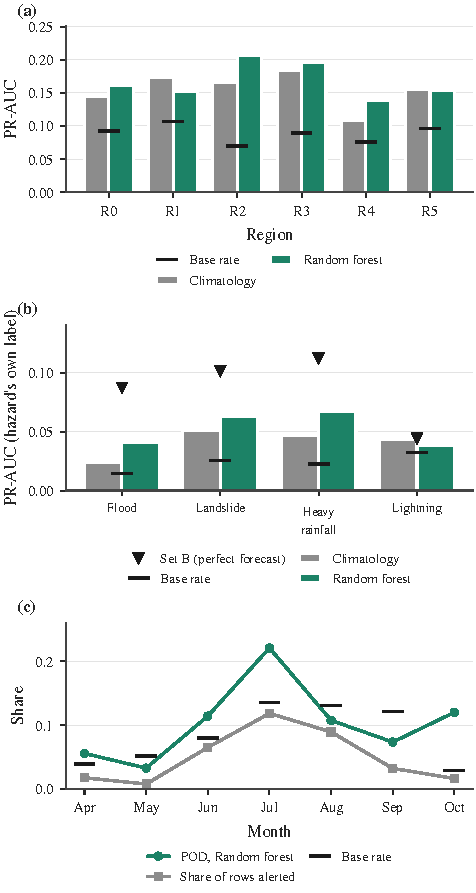
\includegraphics[width=\columnwidth]{fig-errors-region-hazard-month.pdf}
\caption{Random forest (set A, fixed split) on test 2024 to 2025. (a) PR-AUC by region against climatology, with base rates. (b) PR-AUC against each hazard's own label, with the set B ceiling. (c) POD and share of rows alerted by month at the 5\% budget.}
\label{fig:errors}
\end{figure}

\begin{table}[!t]
\caption{PR-AUC on test 2024 to 2025 by feature set (fixed split), with paired differences and 95\% intervals.}
\label{tab:fsets}
\centering
\scriptsize
\setlength{\tabcolsep}{2pt}
\begin{tabular}{lrrrll}
\toprule
Model & NOWX & A & B & A $-$ NOWX [95\% CI] & B $-$ A [95\% CI] \\
\midrule
LR & 0.164 & 0.177 & 0.212 & +0.014 [-0.005, +0.041] & +0.035 [+0.009, +0.072] \\
RF & 0.143 & 0.165 & 0.219 & +0.022 [+0.001, +0.045] & +0.054 [+0.014, +0.112] \\
HGB & 0.164 & 0.175 & 0.220 & +0.011 [-0.007, +0.030] & +0.045 [+0.010, +0.099] \\
SVM-L & 0.164 & 0.177 & 0.211 & +0.013 [-0.007, +0.040] & +0.034 [+0.009, +0.071] \\
SVM-RBF & 0.141 & 0.153 & 0.179 & +0.012 [-0.001, +0.030] & +0.026 [+0.009, +0.051] \\
\bottomrule
\end{tabular}

\end{table}


\clearpage
\section*{Acknowledgment}
Incident data are from the BIPAD portal of the National Disaster Risk Reduction and Management Authority, Government of Nepal. Weather and elevation data are from Open-Meteo (CC BY 4.0), based on ERA5 from the Copernicus Climate Change Service and the Copernicus DEM. Administrative boundaries are from OCHA through the Humanitarian Data Exchange (CC BY-IGO). The analysis used Python 3.12 with scikit-learn, pandas, NumPy, GeoPandas, matplotlib, seaborn and SHAP in Jupyter notebooks, with the environment managed by uv.

\bibliographystyle{IEEEtran}
\bibliography{references}

\end{document}
